\documentclass[../../main.tex]{subfiles}
\begin{document}

{\bf [解]}

\paragraph{(1)} 

\begin{figure}[htb]
 \begin{center}
\begin{tikzpicture}[scale=1.3, >=stealth]

  % --- 1. 座標軸の描画 ---
  \draw[->, thick] (-0.3,0) -- (5.5,0) node[right] {$x$};
  \draw[->, thick] (0,-0.3) -- (0,5.5) node[above] {$y$};
  \node[below left] at (0,0) {$O$};

  % --- 2. x軸・y軸の中略記号 (波線・省略記号) ---
  % x軸の中略
  \draw[thick, white, fill=white] (1.0,-0.15) rectangle (1.4,0.15);
  \draw[thick] (1.0,-0.1) -- (1.2,0.1) -- (1.2,-0.1) -- (1.4,0.1);

  % y軸の中略
  \draw[thick, white, fill=white] (-0.15,1.0) rectangle (0.15,1.4);
  \draw[thick] (-0.1,1.0) -- (0.1,1.2) -- (-0.1,1.2) -- (0.1,1.4);

  % --- 3. 境界 n の点線と領域表示 ---
  % x = n, y = n の境界線（これより内側が k<n, l<n）
  \draw[dashed, gray!50] (4.8,0) -- (4.8,5.0) node[above, black, font=\small] {$x=n$};
  \draw[dashed, gray!50] (0,4.8) -- (5.0,4.8) node[right, black, font=\small] {$y=n$};

  % --- 4. 補助点線ガイド (格子) ---
  \draw[dotted, gray!70] (2.5,0) -- (2.5,4.0);
  \draw[dotted, gray!70] (4.0,0) -- (4.0,4.0);
  \draw[dotted, gray!70] (0,2.5) -- (4.0,2.5);
  \draw[dotted, gray!70] (0,4.0) -- (4.0,4.0);

  % --- 5. (k,l) への遷移矢印 (確率 1/2 の枝分かれ) ---
  % (k-1, l) -> (k, l) : 右移動
  \draw[->, ultra thick, blue!80!black] (2.6, 4.0) -- (3.85, 4.0) 
    node[midway, above, font=\small] {$\frac{1}{2}$};

  % (k, l-1) -> (k, l) : 上移動
  \draw[->, ultra thick, blue!80!black] (4.0, 2.6) -- (4.0, 3.85) 
    node[midway, right, font=\small] {$\frac{1}{2}$};

  % (k, l) からの次の移動 (参考点線矢印)
  \draw[->, dashed, thick, gray] (4.15, 4.0) -- (4.6, 4.0) node[above, font=\tiny] {$\frac{1}{2}$};
  \draw[->, dashed, thick, gray] (4.0, 4.15) -- (4.0, 4.6) node[right, font=\tiny] {$\frac{1}{2}$};

  % --- 6. 格子点のプロット (黒丸・赤丸) とラベル ---
  % 流入元の点
  \fill[black] (2.5, 4.0) circle (2pt) node[above left, font=\small] {$(k-1, l)$};
  \fill[black] (4.0, 2.5) circle (2pt) node[below right, font=\small] {$(k, l-1)$};

  % 目的の点 (k, l) を強調
  \fill[red!80!black] (4.0, 4.0) circle (2.5pt) node[above left, red!80!black, font=\small] {$P(k, l)$};

  % --- 7. 軸の目盛りラベル ---
  \node[below] at (2.5, 0) {$k-1$};
  \node[below] at (4.0, 0) {$k$};
  \node[below] at (4.8, 0) {$n$};

  \node[left] at (0, 2.5) {$l-1$};
  \node[left] at (0, 4.0) {$l$};
  \node[left] at (0, 4.8) {$n$};

\end{tikzpicture}
\caption{$(k,l)$に関連する推移の様子}
 \end{center}
\end{figure}

点$A$が$(k,l)$を通過するのは$k+l$回目の移動の時だけであるからこの場合だけを考えれれば良い．
$k,l \le n-1$の時は各回の移動で点Aは(i)に従う．すなわち$x$方向へ$1$移動するか$y$方向へ$1$移動するかである．
$k+l$回の移動のうち何回目に上へ移動するかかんがえて，
\begin{align}
  P(k,l)={}_{k+l}C_k\left(\dfrac{1}{2}\right)^{k+l}
\end{align}
である．


\paragraph{(2)} 

\begin{figure}[htb]
 \begin{center}
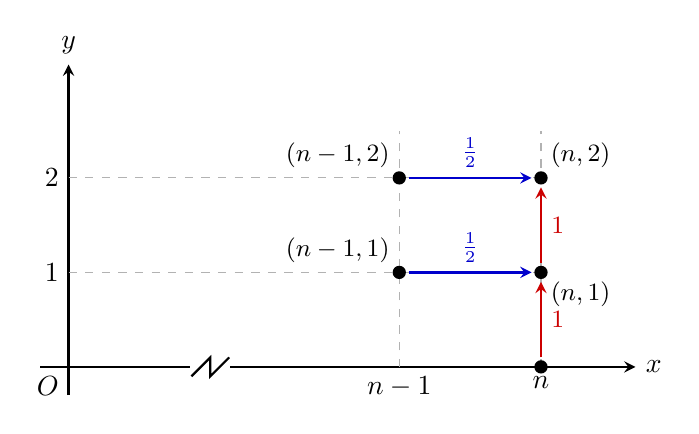
\begin{tikzpicture}[scale=1.2, >=stealth]

  % --- 1. 座標軸の描画 ---
  \draw[->, thick] (-0.3,0) -- (6.0,0) node[right] {$x$};
  \draw[->, thick] (0,-0.3) -- (0,3.2) node[above] {$y$};
  \node[below left] at (0,0) {$O$};

  % --- 2. x軸の中略記号 (波線・省略記号) ---
  % 手書きスケッチにある x 軸上の省略記号
  \draw[thick, white, fill=white] (1.3,-0.15) rectangle (1.7,0.15);
  \draw[thick] (1.3,-0.1) -- (1.5,0.1) -- (1.5,-0.1) -- (1.7,0.1);

  % --- 3. 補助点線ガイド (手書き図の点線) ---
  % y = 1, y = 2 の補助線
  \draw[dashed, gray!60] (0,1) -- (5.0,1);
  \draw[dashed, gray!60] (0,2) -- (5.0,2);
  
  % x = n-1, x = n の補助線
  \draw[dashed, gray!60] (3.5,0) -- (3.5,2.5);
  \draw[dashed, gray!60] (5.0,0) -- (5.0,2.5);

  % --- 4. 遷移の矢印 (確率移動の関係を示示) ---
  % (n-1, 1) -> (n, 1) [確率 1/2]
  \draw[->, thick, blue!80!black] (3.6,1) -- (4.9,1) node[midway, above, font=\small] {$\frac{1}{2}$};
  
  % (n, 0) -> (n, 1) [確率 1]
  \draw[->, thick, red!80!black] (5.0,0.1) -- (5.0,0.9) node[midway, right, font=\small] {$1$};

  % (n-1, 2) -> (n, 2) [確率 1/2]
  \draw[->, thick, blue!80!black] (3.6,2) -- (4.9,2) node[midway, above, font=\small] {$\frac{1}{2}$};

  % (n, 1) -> (n, 2) [確率 1]
  \draw[->, thick, red!80!black] (5.0,1.1) -- (5.0,1.9) node[midway, right, font=\small] {$1$};

  % --- 5. 格子点のプロット (黒丸) とラベル ---
  % 点 (n-1, 1), (n-1, 2)
  \fill[black] (3.5,1) circle (2pt) node[above left, font=\small] {$(n-1,1)$};
  \fill[black] (3.5,2) circle (2pt) node[above left, font=\small] {$(n-1,2)$};

  % 点 (n, 0), (n, 1), (n, 2)
  \fill[black] (5.0,0) circle (2pt);
  \fill[black] (5.0,1) circle (2pt) node[below right, font=\small] {$(n,1)$};
  \fill[black] (5.0,2) circle (2pt) node[above right, font=\small] {$(n,2)$};

  % --- 6. 軸の目盛りラベル ---
  % x軸目盛り
  \node[below] at (3.5,0) {$n-1$};
  \node[below] at (5.0,0) {$n$};

  % y軸目盛り
  \node[left] at (0,1) {$1$};
  \node[left] at (0,2) {$2$};

\end{tikzpicture}
\caption{$x=n$に関連する推移の様子．}
 \end{center}
\end{figure}


題意の法則により
\begin{align}
\begin{split}
  P(n,2)&=P(n,1)+\dfrac{1}{2}P(n-1,2) \quad\cdots\text{①} \\
  P(n,1)&=P(n,0)+\dfrac{1}{2}P(n-1,1) \quad\cdots\text{②}
\end{split} \label{eq:1}
\end{align}
と書けるから右辺を計算することで左辺の$P(n,2)$を求める．

まず$P(n,0)$は$n$回とも右へ移動した場合だから
\begin{align}
 P(n,0)=\left(\dfrac{1}{2}\right)^n \label{eq:2}
\end{align}
である．
$P(n-1,2), P(n-1,2)$は(1)の結果から
\begin{align}
 \begin{cases}
   P(n-1,2)={}_{n+1}C_2\left(\dfrac{1}{2}\right)^{n+1} = n(n+1)\left(\dfrac{1}{2}\right)^{n+2}\\
   P(n-1,1)={}_nC_1\left(\dfrac{1}{2}\right)^n = n\left(\dfrac{1}{2}\right)^n
 \end{cases} \label{eq:3}
\end{align}
である．したがって\cref{eq:2,eq:3}を\cref{eq:1}に代入して
\begin{align}
\begin{split}
P(n,1)&=\left(\dfrac{1}{2}\right)^n+\dfrac{n}{2}\left(\dfrac{1}{2}\right)^n \\
P(n,2)&=\left(1+\dfrac{n}{2}\right)\left(\dfrac{1}{2}\right)^n+\dfrac{1}{2}\cdot\dfrac{(n+1)n}{2}\left(\dfrac{1}{2}\right)^{n+1} \\
&=\dfrac{n^2+5n+8}{8}\left(\dfrac{1}{2}\right)^n
\end{split}
\end{align}
である．



\end{document}
